%\documentclass[mathserif
, handout
]{beamer}
 
 % \useoutertheme{wuerzburg}
%  \useinnertheme[outline]{chamfered}

\usepackage{tabu}
\usepackage{rotating}
\usepackage[]{algorithm2e}
\usepackage{color, colortbl}
%\usepackage{default}
\usepackage{fontspec}
\usepackage{polyglossia} 
\setmainlanguage{vietnamese}
%\setdefaultlanguage{vietnamese} 
%\setmainfont{Palatino}
 \usepackage{wasysym}
\usepackage{pifont}% http://ctan.org/pkg/pifont

\usepackage{multicol}
\usepackage{sidecap}

\usepackage{hyperref}

\usepackage{pgf}    
\usepackage{tikz}
\usetikzlibrary{arrows,automata,decorations.pathmorphing,backgrounds,positioning,fit}
\usepackage{array}
\usepackage{listings}

\usepackage{enumerate}
%\usepackage{amsmath,mathtools}
%		\usepackage{fink}

\usepackage{amsmath,amsthm, amssymb}
\usepackage{microtype}
\usetikzlibrary{arrows,automata}
\usetikzlibrary{decorations.pathmorphing}


\usetikzlibrary{calc}

 

\usetikzlibrary{trees}
\usepackage{listings}

\setbeamertemplate{footline}[frame number]
\setbeamertemplate{navigation symbols}{}%remove navigation symbols

%\usepackage{listingsutf8}

%\setbeameroption{show notes on second screen=right}


  
%\newtheorem{Lemme}{Bổ đề} 
%\newtheorem*{LI}{Lemme d'itération infinie}

%\newtheorem{Proposition}{Mệnh đề}[section]
%\newtheorem{Theorem}{Định lý}[section]
%\newtheorem{Corollaire}{Hệ quả}[section]
%\newtheorem*{Conjecture}{Giả thuyết}
% \newtheorem*{Probleme}{Bài toán}
% \newtheorem*{Fait}{Fait}
% 
% 
% \theoremstyle{definition} \newtheorem{Definition}{Định nghĩa}
% \theoremstyle{definition} \newtheorem{example}{Ví dụ}
% \theoremstyle{remark} \newtheorem*{Remarque}{Chú ý}


\usetikzlibrary{arrows,automata}



\usetikzlibrary{trees}


% \newcommand{\mnvect}[2]
% {
%   \begin{bmatrix}	#1\\#2
%   \end{bmatrix}
% }

\definecolor{olive}{rgb}{0.3, 0.4, .1}
\definecolor{fore}{RGB}{249,242,215}
\definecolor{back}{RGB}{51,51,51}
\definecolor{title}{RGB}{255,0,90}
\definecolor{dgreen}{rgb}{0.,0.7,0. }
\definecolor{gold}{rgb}{1.,0.84,0.}
\definecolor{JungleGreen}{cmyk}{0.99,0,0.52,0}
\definecolor{BlueGreen}{cmyk}{0.85,0,0.37,0}
\definecolor{RawSienna}{cmyk}{0,0.72,1,0.45}
\definecolor{Magenta}{cmyk}{0,1,0,0} 



%

%\setlength{\topmargin}{0cm} \setlength{\oddsidemargin}{0cm}
%\setlength{\evensidemargin}{0cm} \setlength{\textwidth}{17truecm}
%\setlength{\textheight}{21.0truecm}


%\parindent = 3 pt
%\parskip = 12 pt

%\newtheorem*{LI}{Lemme d'itération infinie}



\newtheorem{prprt}{Propriété}
\newtheorem{prpstn}{Mệnh đề}
\newtheorem{thrm}{Định lý}
\newtheorem{lmm}{Bổ đề}

\newtheorem{crllr}{Hệ quả}
\newtheorem{clm}{Fait}
\newtheorem{nt}{Notation}
 
\newtheorem*{cnjctr}{Conjecture}
\newtheorem{prblm}{Problème}
\newtheorem{qstn}{Question}
\newtheorem{fct}{Fait}
%\newtheorem{xmpl}{Exemple}
\newtheorem{rmrk}{Nhận xét}

\theoremstyle{example}
\newtheorem{xmpl}{Ví dụ}
\newtheorem{xrcs}{Bài tập}
  \newtheorem{dfntn}{Định nghĩa}
  

% \declaretheorem[name=Problème]{prblm}
% \declaretheorem[name=Question, style=remark, numbered=no]{qstn}

% \declaretheorem[name=Théorème, numberwithin=section]{thrm}
% \declaretheorem[name=Lemme, sibling=thrm]{lmm}
% \declaretheorem[ name=Propriété, sibling=thrm]{prprt}
% \declaretheorem[ name=Proposition, sibling=thrm]{prpstn}
% \declaretheorem[name=Corollaire, sibling=thrm]{crllr}
% \declaretheorem[name=Fait, sibling=thrm]{fct}
% \declaretheorem[name=Notation, sibling=thrm]{nt}


% \declaretheorem[style=definition, name=Définition, sibling=thrm]{dfntn}

% %\theoremstyle{definition} \newtheorem{dfntn}{Définition}[section]

% \renewcommand\thmcontinues[1]{reprise de p.\,\pageref{#1}}

% \declaretheorem[style=remark, name=Exemple%, numberwithin=section
% ]{xmpl}

% \declaretheorem[style=remark, name=Remarque, numbered=no]{rmrk}

% %\declaretheorem[style=definition,numberwithin=chapter,name = Exemple]{xmpl}

% %\theoremstyle{remark} \newtheorem{xmpl}{Exemple}[chapter]

% %\theoremstyle{remark} \newtheorem*{rmrk}{Remarque}



\newtheorem{cs}{Cas}


\def\mclose{\texttt{close}}
\def\mopen{\texttt{open}}

\def\mmclose{\texttt{\scriptsize close}}
\def\mmopen{\texttt{\scriptsize open}}



% \newcommand{\mvect}[2]
% {
% \bigl[ \begin{smallmatrix}
% #1\\ #2
% \end{smallmatrix} \bigr]
% }

% \newcommand{\mnvect}[2]
% {
%   \begin{bmatrix}	#1\\#2
%   \end{bmatrix}
% }

% % \newcommand{\mnvect}[2]
% % {
% % #1/#2
% %   % \begin{bmatrix}	#1\\#2
% %   % \end{bmatrix}
% % }

% \newcommand{\XMPL}[3]
% {
%   \begin{xmpl}
%     Soient $L=\{#1\}$ et $\Sigma=\{#2\}$. On peut vérifier que $L$ est \orl\ avec le
%     relateur de base $#3$.
%   \end{xmpl}
% }

% \newcommand{\XMP}[4]
% {
%   \begin{xmpl}[#4]
%     Soient $L=\{#1\}$ et $\Sigma=\{#2\}$. On peut vérifier que $L$ est \orl\ avec le
%     relateur de base $#3$.
%   \end{xmpl}
% }

% \newcommand{\Pui}[2]
% {
%   #1^{\leq #2}
% }


% % \newcommand{\XMPL1}[4]
% % {
% %   \begin{xmpl}
% %     Soient $L=\{#1\}$ et $\Sigma=\{#2\}$. Il est clair que $L$ est \orl\ avec le
% %     relateur de base $#3$. $L^\omega$ est un 
% %   \end{xmpl}
% % }

% \def\vvs{\vspace{11pt}}
% \def\nni{\noindent}


% \newcommand{\cas}[1]
% {
% \vvs\nni
% \textbf{Cas #1 :}
% }



% \newcommand{\souscas}[1]
% {
% \vvs\nni
% \textbf{Sous-cas #1 :}
% }

% \def\pcom{paire de mots incompatibles}
% \def\wpcom{paire de mots $\infty$-incompatible}

% \def\upcom{une paire de mots incompatibles}
% \def\uwpcom{une paire de mots $\infty$-incompatibles}
% \def\comp{\asymp}

% \def\wg{code générateur}

%  \def\gc{code générateur}

% \def\gcx{codes générateurs}
% \def\Gcx{Codes générateurs }
% \def\ugc{un code générateur}
% \def\Ugc{un Code générateur}

% \def\wgc{$\omega$-code générateur}
% \def\wgcx{$\omega$-codes générateurs}
% \def\wGcx{$\omega$-Codes générateurs }
% \def\wugc{un $\omega$-code générateur}
% \def\wUgc{un $\omega$-code générateur}

% \def\orl {langage à un relateur}

% \def\orlx {langages à un relateur}
% \def\Orlx {Langages à un relateur}
% \def\uorl {un langage à un relateur}


% \def\ugc{un code générateur}

% \def\cp{code préfixe}

% \def\iff{si et seulement si} 
% \def\w{\omega}

% \def\CODE{la proposition~\ref{c3prop23}, $L^\omega$ n'a pas de \gc}
% \def\NOCODE{$L^\omega$ n'a pas de \gc}


\def\vs{}
\def\ni{}





%\setlength{\topmargin}{0cm} \setlength{\oddsidemargin}{0cm}
%\setlength{\evensidemargin}{0cm} \setlength{\textwidth}{17truecm}
%\setlength{\textheight}{21.0truecm}


%\parindent = 3 pt
%\parskip = 12 pt

%\newtheorem*{LI}{Lemme d'itération infinie}



\newtheorem{prprt}{Propriété}
\newtheorem{prpstn}{Mệnh đề}
\newtheorem{thrm}{Định lý}
\newtheorem{lmm}{Bổ đề}
\newtheorem{rl}{Luật}

\newtheorem{crllr}{Hệ quả}
\newtheorem{clm}{Khẳng định}
\newtheorem{nt}{Notation}
 
\newtheorem*{cnjctr}{Giả thuyết}

\newtheorem{fct}{Fait}
%\newtheorem{xmpl}{Exemple}

\theoremstyle{example}
\newtheorem{xmpl}{Ví dụ}
\newtheorem{xrcs}{Bài tập}
  \newtheorem{dfntn}{Định nghĩa}
  \newtheorem{qstn}{Câu hỏi}
\newtheorem{prblm}{Bài toán}  
   \newtheorem{sol}{Lời giải}
\newtheorem{rmrk}{Nhận xét}
  
%  \newtheorem{rmrk}{Định nghĩa}
  

% \declaretheorem[name=Problème]{prblm}
% \declaretheorem[name=Question, style=remark, numbered=no]{qstn}

% \declaretheorem[name=Théorème, numberwithin=section]{thrm}
% \declaretheorem[name=Lemme, sibling=thrm]{lmm}
% \declaretheorem[ name=Propriété, sibling=thrm]{prprt}
% \declaretheorem[ name=Proposition, sibling=thrm]{prpstn}
% \declaretheorem[name=Corollaire, sibling=thrm]{crllr}
% \declaretheorem[name=Fait, sibling=thrm]{fct}
% \declaretheorem[name=Notation, sibling=thrm]{nt}


% \declaretheorem[style=definition, name=Définition, sibling=thrm]{dfntn}

% %\theoremstyle{definition} \newtheorem{dfntn}{Définition}[section]

% \renewcommand\thmcontinues[1]{reprise de p.\,\pageref{#1}}

% \declaretheorem[style=remark, name=Exemple%, numberwithin=section
% ]{xmpl}

% \declaretheorem[style=remark, name=Remarque, numbered=no]{rmrk}

% %\declaretheorem[style=definition,numberwithin=chapter,name = Exemple]{xmpl}

% %\theoremstyle{remark} \newtheorem{xmpl}{Exemple}[chapter]

% %\theoremstyle{remark} \newtheorem*{rmrk}{Remarque}



\newtheorem{cs}{Cas}


\def\mclose{\texttt{close}}
\def\mopen{\texttt{open}}

\def\mmclose{\texttt{\scriptsize close}}
\def\mmopen{\texttt{\scriptsize open}}



% \newcommand{\mvect}[2]
% {
% \bigl[ \begin{smallmatrix}
% #1\\ #2
% \end{smallmatrix} \bigr]
% }

% \newcommand{\mnvect}[2]
% {
%   \begin{bmatrix}	#1\\#2
%   \end{bmatrix}
% }

% % \newcommand{\mnvect}[2]
% % {
% % #1/#2
% %   % \begin{bmatrix}	#1\\#2
% %   % \end{bmatrix}
% % }

% \newcommand{\XMPL}[3]
% {
%   \begin{xmpl}
%     Soient $L=\{#1\}$ et $\Sigma=\{#2\}$. On peut vérifier que $L$ est \orl\ avec le
%     relateur de base $#3$.
%   \end{xmpl}
% }

% \newcommand{\XMP}[4]
% {
%   \begin{xmpl}[#4]
%     Soient $L=\{#1\}$ et $\Sigma=\{#2\}$. On peut vérifier que $L$ est \orl\ avec le
%     relateur de base $#3$.
%   \end{xmpl}
% }

% \newcommand{\Pui}[2]
% {
%   #1^{\leq #2}
% }


% % \newcommand{\XMPL1}[4]
% % {
% %   \begin{xmpl}
% %     Soient $L=\{#1\}$ et $\Sigma=\{#2\}$. Il est clair que $L$ est \orl\ avec le
% %     relateur de base $#3$. $L^\omega$ est un 
% %   \end{xmpl}
% % }

% \def\vvs{\vspace{11pt}}
% \def\nni{\noindent}


% \newcommand{\cas}[1]
% {
% \vvs\nni
% \textbf{Cas #1 :}
% }



% \newcommand{\souscas}[1]
% {
% \vvs\nni
% \textbf{Sous-cas #1 :}
% }

% \def\pcom{paire de mots incompatibles}
% \def\wpcom{paire de mots $\infty$-incompatible}

% \def\upcom{une paire de mots incompatibles}
% \def\uwpcom{une paire de mots $\infty$-incompatibles}
% \def\comp{\asymp}

% \def\wg{code générateur}

%  \def\gc{code générateur}

% \def\gcx{codes générateurs}
% \def\Gcx{Codes générateurs }
% \def\ugc{un code générateur}
% \def\Ugc{un Code générateur}

% \def\wgc{$\omega$-code générateur}
% \def\wgcx{$\omega$-codes générateurs}
% \def\wGcx{$\omega$-Codes générateurs }
% \def\wugc{un $\omega$-code générateur}
% \def\wUgc{un $\omega$-code générateur}

% \def\orl {langage à un relateur}

% \def\orlx {langages à un relateur}
% \def\Orlx {Langages à un relateur}
% \def\uorl {un langage à un relateur}


% \def\ugc{un code générateur}

% \def\cp{code préfixe}

% \def\iff{si et seulement si} 
% \def\w{\omega}

% \def\CODE{la proposition~\ref{c3prop23}, $L^\omega$ n'a pas de \gc}
% \def\NOCODE{$L^\omega$ n'a pas de \gc}


\def\vs{}
\def\ni{}


\def\trail{hành trình đơn}
\def\Trail{Hành trình đơn}

\def\ctrail{\trail\ đóng}
\def\Ctrail{\Trail\ đóng }

\def\walk{hành trình}
\def\Walk{Hành trình}

\def\cwalk{hành trình đóng}
\def\Cwalk{Hành trình đóng}

\def\path{đường đi}
\def\Path{Đường đi}
 
\def\conn{liên thông}
\def\Conn{Liên thông}

\def\Comp{Thành phần liên thông}
\def\comp{thành phần liên thông}

\def\Cuted{Cạnh cắt}
\def\cuted{cạnh cắt}

\def\Cutve{Đỉnh cắt}
\def\cutve{đỉnh cắt}

\def\Induced{Đồ thị con cảm sinh}
\def\induced{đồ thị con cảm sinh}

 
\def\iff{{\color{blue} nếu và chỉ nếu}}

\def\ideg{\text{indeg}}
\def\odeg{\text{outdeg}}

\def\pr{\mathrm{Pr}}
\def\ex{\mathrm{Ex}}
\def\S{\mathcal{S}}
\def\var{\mathrm{Var}}

\def\F{\mathbb{F}}
\def\Z{\mathbb{Z}}
\def\N{\mathbb{N}}
\def\ord{\mathrm{ord}}
\newcommand{\bigO}{\ensuremath{\mathcal{O}}}% big-O notation/symbol


 \newcommand{\defi}[1]{{\color{blue}{\textbf{\emph{#1}}}}}
\newcommand{\contradiction}{{\hbox{%
    \setbox0=\hbox{$\mkern-3mu\times\mkern-3mu$}%
    \setbox1=\hbox to0pt{\hss$\times$\hss}%
    \copy0\raisebox{0.5\wd0}{\copy1}\raisebox{-0.5\wd0}{\box1}\box0
}}}

\newcommand{\cmark}{{\color{blue}\Large\ding{51}}}%
\newcommand{\xmark}{{\color{red}\Large\ding{55}}}%

%\newcommand{\defi}[1]{{\color{blue}{\textbf{\emph{#1}}}}}


 \AtBeginSection[]  
 { 
   \begin{frame}[plain]{Nội dung} 
     \tableofcontents[currentsection,currentsubsection] 
   \end{frame} 
 }  



\begin{document}
% \tikzstyle{every picture}+=[remember picture]

% \tikzstyle{na} = [baseline=-.5ex]

\author{Trần Vĩnh Đức}
%\institute[HUST]{Hanoi University of Science and Technology}


\documentclass[mathserif
%, handout
]{beamer}
 
  \useoutertheme{wuerzburg}
  \useinnertheme[outline]{chamfered}
 \usecolortheme{shark}
 \definecolor{MyBackground}{RGB}{243,246,249}
 \setbeamercolor{background canvas}{bg=MyBackground}

 %\usecolortheme[snowy]{owl}
 %\usecolortheme{owl}
 
 %\usetheme{Warsaw}
 %\usecolortheme{spruce}

\usepackage{tabu}
\usepackage{rotating}
\usepackage[]{algorithm2e}
\usepackage{color, colortbl}
%\usepackage{default}
\usepackage{fontspec}
\usepackage{polyglossia} 
\setmainlanguage{vietnamese}
%\setdefaultlanguage{vietnamese} 
%\setmainfont{Palatino}
 \usepackage{wasysym}
\usepackage{pifont}% http://ctan.org/pkg/pifont

\usepackage{multicol}
\usepackage{sidecap}

\usepackage{hyperref}

\usepackage{pgf}    
\usepackage{tikz}
\usetikzlibrary{arrows,automata,decorations.pathmorphing,backgrounds,positioning,fit}
\usepackage{array}
\usepackage{listings}

\usepackage{enumerate}
%\usepackage{amsmath,mathtools}
%		\usepackage{fink}

\usepackage{amsmath,amsthm, amssymb}
\usepackage{microtype}
\usetikzlibrary{arrows,automata}
\usetikzlibrary{decorations.pathmorphing}


\usetikzlibrary{calc}

 

\usetikzlibrary{trees}
\usepackage{listings}

\setbeamertemplate{footline}[frame number]
\setbeamertemplate{navigation symbols}{}%remove navigation symbols

%\usepackage{listingsutf8}

%\setbeameroption{show notes on second screen=right}


  
%\newtheorem{Lemme}{Bổ đề} 
%\newtheorem*{LI}{Lemme d'itération infinie}

%\newtheorem{Proposition}{Mệnh đề}[section]
%\newtheorem{Theorem}{Định lý}[section]
%\newtheorem{Corollaire}{Hệ quả}[section]
%\newtheorem*{Conjecture}{Giả thuyết}
% \newtheorem*{Probleme}{Bài toán}
% \newtheorem*{Fait}{Fait}
% 
% 
% \theoremstyle{definition} \newtheorem{Definition}{Định nghĩa}
% \theoremstyle{definition} \newtheorem{example}{Ví dụ}
% \theoremstyle{remark} \newtheorem*{Remarque}{Chú ý}


\usetikzlibrary{arrows,automata}



\usetikzlibrary{trees}


% \newcommand{\mnvect}[2]
% {
%   \begin{bmatrix}	#1\\#2
%   \end{bmatrix}
% }

\definecolor{olive}{rgb}{0.3, 0.4, .1}
\definecolor{fore}{RGB}{249,242,215}
\definecolor{back}{RGB}{51,51,51}
\definecolor{title}{RGB}{255,0,90}
\definecolor{dgreen}{rgb}{0.,0.7,0. }
\definecolor{gold}{rgb}{1.,0.84,0.}
\definecolor{JungleGreen}{cmyk}{0.99,0,0.52,0}
\definecolor{BlueGreen}{cmyk}{0.85,0,0.37,0}
\definecolor{RawSienna}{cmyk}{0,0.72,1,0.45}
\definecolor{Magenta}{cmyk}{0,1,0,0} 



%

%\setlength{\topmargin}{0cm} \setlength{\oddsidemargin}{0cm}
%\setlength{\evensidemargin}{0cm} \setlength{\textwidth}{17truecm}
%\setlength{\textheight}{21.0truecm}


%\parindent = 3 pt
%\parskip = 12 pt

%\newtheorem*{LI}{Lemme d'itération infinie}



\newtheorem{prprt}{Propriété}
\newtheorem{prpstn}{Mệnh đề}
\newtheorem{thrm}{Định lý}
\newtheorem{lmm}{Bổ đề}

\newtheorem{crllr}{Hệ quả}
\newtheorem{clm}{Fait}
\newtheorem{nt}{Notation}
 
\newtheorem*{cnjctr}{Conjecture}
\newtheorem{prblm}{Problème}
\newtheorem{qstn}{Question}
\newtheorem{fct}{Fait}
%\newtheorem{xmpl}{Exemple}
\newtheorem{rmrk}{Nhận xét}

\theoremstyle{example}
\newtheorem{xmpl}{Ví dụ}
\newtheorem{xrcs}{Bài tập}
  \newtheorem{dfntn}{Định nghĩa}
  

% \declaretheorem[name=Problème]{prblm}
% \declaretheorem[name=Question, style=remark, numbered=no]{qstn}

% \declaretheorem[name=Théorème, numberwithin=section]{thrm}
% \declaretheorem[name=Lemme, sibling=thrm]{lmm}
% \declaretheorem[ name=Propriété, sibling=thrm]{prprt}
% \declaretheorem[ name=Proposition, sibling=thrm]{prpstn}
% \declaretheorem[name=Corollaire, sibling=thrm]{crllr}
% \declaretheorem[name=Fait, sibling=thrm]{fct}
% \declaretheorem[name=Notation, sibling=thrm]{nt}


% \declaretheorem[style=definition, name=Définition, sibling=thrm]{dfntn}

% %\theoremstyle{definition} \newtheorem{dfntn}{Définition}[section]

% \renewcommand\thmcontinues[1]{reprise de p.\,\pageref{#1}}

% \declaretheorem[style=remark, name=Exemple%, numberwithin=section
% ]{xmpl}

% \declaretheorem[style=remark, name=Remarque, numbered=no]{rmrk}

% %\declaretheorem[style=definition,numberwithin=chapter,name = Exemple]{xmpl}

% %\theoremstyle{remark} \newtheorem{xmpl}{Exemple}[chapter]

% %\theoremstyle{remark} \newtheorem*{rmrk}{Remarque}



\newtheorem{cs}{Cas}


\def\mclose{\texttt{close}}
\def\mopen{\texttt{open}}

\def\mmclose{\texttt{\scriptsize close}}
\def\mmopen{\texttt{\scriptsize open}}



% \newcommand{\mvect}[2]
% {
% \bigl[ \begin{smallmatrix}
% #1\\ #2
% \end{smallmatrix} \bigr]
% }

% \newcommand{\mnvect}[2]
% {
%   \begin{bmatrix}	#1\\#2
%   \end{bmatrix}
% }

% % \newcommand{\mnvect}[2]
% % {
% % #1/#2
% %   % \begin{bmatrix}	#1\\#2
% %   % \end{bmatrix}
% % }

% \newcommand{\XMPL}[3]
% {
%   \begin{xmpl}
%     Soient $L=\{#1\}$ et $\Sigma=\{#2\}$. On peut vérifier que $L$ est \orl\ avec le
%     relateur de base $#3$.
%   \end{xmpl}
% }

% \newcommand{\XMP}[4]
% {
%   \begin{xmpl}[#4]
%     Soient $L=\{#1\}$ et $\Sigma=\{#2\}$. On peut vérifier que $L$ est \orl\ avec le
%     relateur de base $#3$.
%   \end{xmpl}
% }

% \newcommand{\Pui}[2]
% {
%   #1^{\leq #2}
% }


% % \newcommand{\XMPL1}[4]
% % {
% %   \begin{xmpl}
% %     Soient $L=\{#1\}$ et $\Sigma=\{#2\}$. Il est clair que $L$ est \orl\ avec le
% %     relateur de base $#3$. $L^\omega$ est un 
% %   \end{xmpl}
% % }

% \def\vvs{\vspace{11pt}}
% \def\nni{\noindent}


% \newcommand{\cas}[1]
% {
% \vvs\nni
% \textbf{Cas #1 :}
% }



% \newcommand{\souscas}[1]
% {
% \vvs\nni
% \textbf{Sous-cas #1 :}
% }

% \def\pcom{paire de mots incompatibles}
% \def\wpcom{paire de mots $\infty$-incompatible}

% \def\upcom{une paire de mots incompatibles}
% \def\uwpcom{une paire de mots $\infty$-incompatibles}
% \def\comp{\asymp}

% \def\wg{code générateur}

%  \def\gc{code générateur}

% \def\gcx{codes générateurs}
% \def\Gcx{Codes générateurs }
% \def\ugc{un code générateur}
% \def\Ugc{un Code générateur}

% \def\wgc{$\omega$-code générateur}
% \def\wgcx{$\omega$-codes générateurs}
% \def\wGcx{$\omega$-Codes générateurs }
% \def\wugc{un $\omega$-code générateur}
% \def\wUgc{un $\omega$-code générateur}

% \def\orl {langage à un relateur}

% \def\orlx {langages à un relateur}
% \def\Orlx {Langages à un relateur}
% \def\uorl {un langage à un relateur}


% \def\ugc{un code générateur}

% \def\cp{code préfixe}

% \def\iff{si et seulement si} 
% \def\w{\omega}

% \def\CODE{la proposition~\ref{c3prop23}, $L^\omega$ n'a pas de \gc}
% \def\NOCODE{$L^\omega$ n'a pas de \gc}


\def\vs{}
\def\ni{}





%\setlength{\topmargin}{0cm} \setlength{\oddsidemargin}{0cm}
%\setlength{\evensidemargin}{0cm} \setlength{\textwidth}{17truecm}
%\setlength{\textheight}{21.0truecm}


%\parindent = 3 pt
%\parskip = 12 pt

%\newtheorem*{LI}{Lemme d'itération infinie}



\newtheorem{prprt}{Propriété}
\newtheorem{prpstn}{Mệnh đề}
\newtheorem{thrm}{Định lý}
\newtheorem{lmm}{Bổ đề}
\newtheorem{rl}{Luật}

\newtheorem{crllr}{Hệ quả}
\newtheorem{clm}{Khẳng định}
\newtheorem{nt}{Notation}
 
\newtheorem*{cnjctr}{Giả thuyết}

\newtheorem{fct}{Fait}
%\newtheorem{xmpl}{Exemple}

\theoremstyle{example}
\newtheorem{xmpl}{Ví dụ}
\newtheorem{xrcs}{Bài tập}
  \newtheorem{dfntn}{Định nghĩa}
  \newtheorem{qstn}{Câu hỏi}
\newtheorem{prblm}{Bài toán}  
   \newtheorem{sol}{Lời giải}
\newtheorem{rmrk}{Nhận xét}
  
%  \newtheorem{rmrk}{Định nghĩa}
  

% \declaretheorem[name=Problème]{prblm}
% \declaretheorem[name=Question, style=remark, numbered=no]{qstn}

% \declaretheorem[name=Théorème, numberwithin=section]{thrm}
% \declaretheorem[name=Lemme, sibling=thrm]{lmm}
% \declaretheorem[ name=Propriété, sibling=thrm]{prprt}
% \declaretheorem[ name=Proposition, sibling=thrm]{prpstn}
% \declaretheorem[name=Corollaire, sibling=thrm]{crllr}
% \declaretheorem[name=Fait, sibling=thrm]{fct}
% \declaretheorem[name=Notation, sibling=thrm]{nt}


% \declaretheorem[style=definition, name=Définition, sibling=thrm]{dfntn}

% %\theoremstyle{definition} \newtheorem{dfntn}{Définition}[section]

% \renewcommand\thmcontinues[1]{reprise de p.\,\pageref{#1}}

% \declaretheorem[style=remark, name=Exemple%, numberwithin=section
% ]{xmpl}

% \declaretheorem[style=remark, name=Remarque, numbered=no]{rmrk}

% %\declaretheorem[style=definition,numberwithin=chapter,name = Exemple]{xmpl}

% %\theoremstyle{remark} \newtheorem{xmpl}{Exemple}[chapter]

% %\theoremstyle{remark} \newtheorem*{rmrk}{Remarque}



\newtheorem{cs}{Cas}


\def\mclose{\texttt{close}}
\def\mopen{\texttt{open}}

\def\mmclose{\texttt{\scriptsize close}}
\def\mmopen{\texttt{\scriptsize open}}



% \newcommand{\mvect}[2]
% {
% \bigl[ \begin{smallmatrix}
% #1\\ #2
% \end{smallmatrix} \bigr]
% }

% \newcommand{\mnvect}[2]
% {
%   \begin{bmatrix}	#1\\#2
%   \end{bmatrix}
% }

% % \newcommand{\mnvect}[2]
% % {
% % #1/#2
% %   % \begin{bmatrix}	#1\\#2
% %   % \end{bmatrix}
% % }

% \newcommand{\XMPL}[3]
% {
%   \begin{xmpl}
%     Soient $L=\{#1\}$ et $\Sigma=\{#2\}$. On peut vérifier que $L$ est \orl\ avec le
%     relateur de base $#3$.
%   \end{xmpl}
% }

% \newcommand{\XMP}[4]
% {
%   \begin{xmpl}[#4]
%     Soient $L=\{#1\}$ et $\Sigma=\{#2\}$. On peut vérifier que $L$ est \orl\ avec le
%     relateur de base $#3$.
%   \end{xmpl}
% }

% \newcommand{\Pui}[2]
% {
%   #1^{\leq #2}
% }


% % \newcommand{\XMPL1}[4]
% % {
% %   \begin{xmpl}
% %     Soient $L=\{#1\}$ et $\Sigma=\{#2\}$. Il est clair que $L$ est \orl\ avec le
% %     relateur de base $#3$. $L^\omega$ est un 
% %   \end{xmpl}
% % }

% \def\vvs{\vspace{11pt}}
% \def\nni{\noindent}


% \newcommand{\cas}[1]
% {
% \vvs\nni
% \textbf{Cas #1 :}
% }



% \newcommand{\souscas}[1]
% {
% \vvs\nni
% \textbf{Sous-cas #1 :}
% }

% \def\pcom{paire de mots incompatibles}
% \def\wpcom{paire de mots $\infty$-incompatible}

% \def\upcom{une paire de mots incompatibles}
% \def\uwpcom{une paire de mots $\infty$-incompatibles}
% \def\comp{\asymp}

% \def\wg{code générateur}

%  \def\gc{code générateur}

% \def\gcx{codes générateurs}
% \def\Gcx{Codes générateurs }
% \def\ugc{un code générateur}
% \def\Ugc{un Code générateur}

% \def\wgc{$\omega$-code générateur}
% \def\wgcx{$\omega$-codes générateurs}
% \def\wGcx{$\omega$-Codes générateurs }
% \def\wugc{un $\omega$-code générateur}
% \def\wUgc{un $\omega$-code générateur}

% \def\orl {langage à un relateur}

% \def\orlx {langages à un relateur}
% \def\Orlx {Langages à un relateur}
% \def\uorl {un langage à un relateur}


% \def\ugc{un code générateur}

% \def\cp{code préfixe}

% \def\iff{si et seulement si} 
% \def\w{\omega}

% \def\CODE{la proposition~\ref{c3prop23}, $L^\omega$ n'a pas de \gc}
% \def\NOCODE{$L^\omega$ n'a pas de \gc}


\def\vs{}
\def\ni{}


\def\trail{hành trình đơn}
\def\Trail{Hành trình đơn}

\def\ctrail{\trail\ đóng}
\def\Ctrail{\Trail\ đóng }

\def\walk{hành trình}
\def\Walk{Hành trình}

\def\cwalk{hành trình đóng}
\def\Cwalk{Hành trình đóng}

\def\path{đường đi}
\def\Path{Đường đi}
 
\def\conn{liên thông}
\def\Conn{Liên thông}

\def\Comp{Thành phần liên thông}
\def\comp{thành phần liên thông}

\def\Cuted{Cạnh cắt}
\def\cuted{cạnh cắt}

\def\Cutve{Đỉnh cắt}
\def\cutve{đỉnh cắt}

\def\Induced{Đồ thị con cảm sinh}
\def\induced{đồ thị con cảm sinh}

 
\def\iff{{\color{blue} nếu và chỉ nếu}}

\def\ideg{\text{indeg}}
\def\odeg{\text{outdeg}}

\def\pr{\mathrm{Pr}}
\def\ex{\mathrm{Ex}}
\def\S{\mathcal{S}}
\def\var{\mathrm{Var}}

\def\F{\mathbb{F}}
\def\Z{\mathbb{Z}}
\def\N{\mathbb{N}}
\def\ord{\mathrm{ord}}
\newcommand{\bigO}{\ensuremath{\mathcal{O}}}% big-O notation/symbol


 \newcommand{\defi}[1]{{\color{blue}{\textbf{\emph{#1}}}}}
\newcommand{\contradiction}{{\hbox{%
    \setbox0=\hbox{$\mkern-3mu\times\mkern-3mu$}%
    \setbox1=\hbox to0pt{\hss$\times$\hss}%
    \copy0\raisebox{0.5\wd0}{\copy1}\raisebox{-0.5\wd0}{\box1}\box0
}}}

\newcommand{\cmark}{{\color{blue}\Large\ding{51}}}%
\newcommand{\xmark}{{\color{red}\Large\ding{55}}}%

%\newcommand{\defi}[1]{{\color{blue}{\textbf{\emph{#1}}}}}


 \AtBeginSection[]  
 { 
   \begin{frame}[plain]{Nội dung} 
     \tableofcontents[currentsection,currentsubsection] 
   \end{frame} 
 }  



\begin{document}
% \tikzstyle{every picture}+=[remember picture]

% \tikzstyle{na} = [baseline=-.5ex]

\author{Trần Vĩnh Đức}
%\institute[HUST]{Hanoi University of Science and Technology}




% \newcommand{\cmark}{{\color{blue}\Large\ding{51}}}%
% \newcommand{\xmark}{{\color{red}\Large\ding{55}}}%
\title{Nhập Môn Xác Suất Rời Rạc} 
 \author{Trần Vĩnh Đức}    
\institute[HUST]{HUST}
 
\maketitle

\begin{frame}{Tài liệu tham khảo}
  \begin{itemize}
  \item Eric Lehman, F Thomson Leighton \& Albert R Meyer,
    \textit{Mathematics for Computer Science}, 2013
    \href{https://www.seas.harvard.edu/courses/cs20/MIT6_042Notes.pdf}{\color{blue}(Miễn
    phí)}
  \item Michael Mitzenmacher và Eli Upfal, \textit{Probability and Computing}, 2005
%  \item Phan .Đ. Diệu, \textit{Logic toán \& cơ sở toán học}. (2003)  
  \end{itemize}
\end{frame}

\section{Trò chơi Monty Hall}
\begin{frame}{Bài toán Monty Hall}
  \begin{itemize}
  \item Có $3$ cánh cửa A,B, và C; đằng sau $1$ trong $3$ cánh cửa đó là một món quà lớn; còn sau hai cửa còn lại không có gì.
  \item Người chơi được chọn $1$ trong $3$ cánh cửa, nếu chọn đúng cửa có quà thì được nhận quà.
  \item Sau khi người chơi đã chọn một cửa, người dẫn chương trình Carol  mở một trong hai cửa còn lại nhưng sẽ chỉ mở cửa không có quà.
  \item Sau đó người chơi được quyền chọn, hoặc là giữ cửa mình chọn ban đầu, hoặc đổi lấy cửa chưa được mở còn lại.
  \item Theo bạn thì người chơi có nên đổi không?
  \end{itemize}
\end{frame}

\begin{frame}{Mô phỏng}
  \href{open /data/Dropbox/Teaching/BachKhoa/Courses/ToanChuyenDe2015/simulation/MontyHall.java}{\beamergotobutton{Source Code:  MontyHall.java}}
\end{frame}
\begin{frame}
  \begin{dfntn}
     \defi{Không gian mẫu}, thường được kí hiệu là $\mathcal{S}$, của một thí nghiệm hay của một phép thử ngẫu nhiên là tập hợp của tất cả các \defi{kết quả} có thể xảy ra. 
  \end{dfntn}

  \begin{xmpl}
    Một kết quả của trò chơi Monty Hall bao gồm:
    \begin{enumerate}
    \item cửa có chứa phần thưởng,
    \item cửa được người chơi chọn, và
    \item cửa được người dẫn chương trình Carol mở.
    \end{enumerate}
  \end{xmpl}
\end{frame}

\begin{frame}
  \begin{xmpl}
    Kết quả $(B, A, C)$ có nghĩa rằng 
    \begin{enumerate}
    \item cửa $B$ có chứa phần thưởng,
    \item người chơi chọn cửa $A$, và
    \item người dẫn chương trình Carol cửa $C$.
    \end{enumerate}
  \end{xmpl}
\end{frame}

\begin{frame}
  \begin{xmpl}
    \begin{itemize}
    \item $(A,B,A)$ không phải là một kết quả.
    \item $(B,A,A)$
    \item $(A,A,B)$
    \item $(A,A,C)$
    \end{itemize}
  \end{xmpl}
\end{frame}

\begin{frame}
   % \begin{center}
      \begin{block}{}
        \begin{center}
          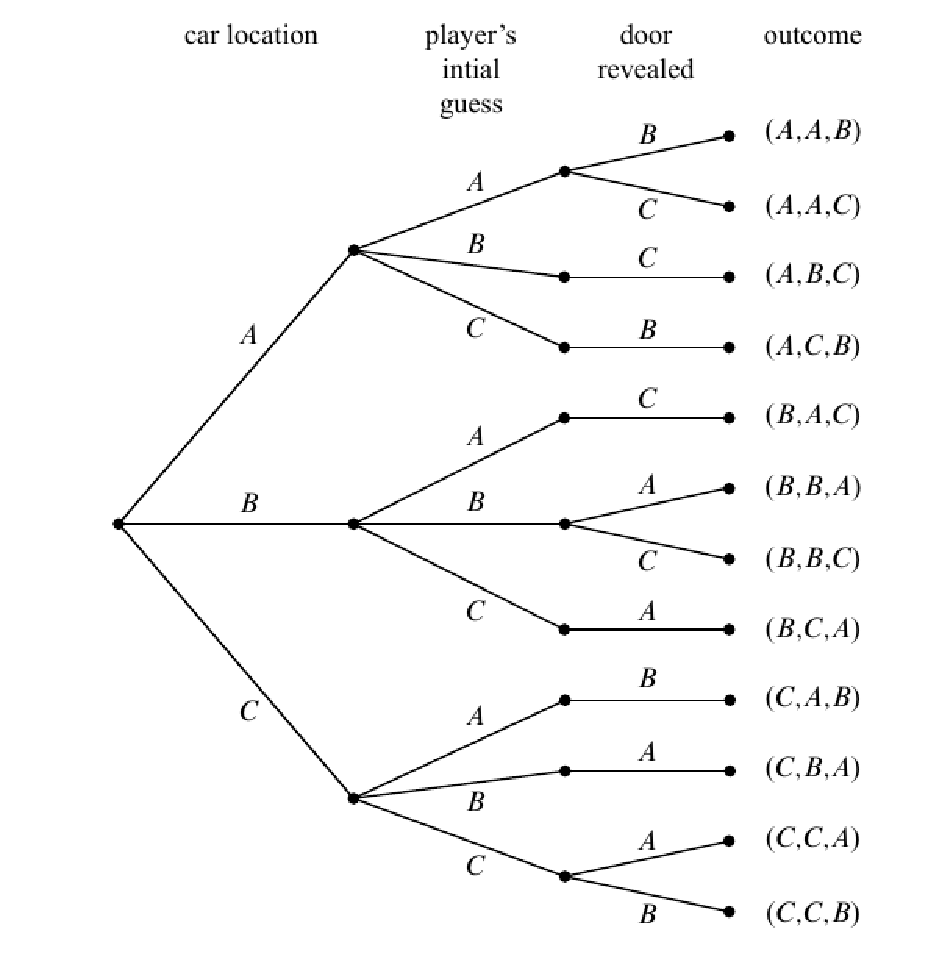
\includegraphics[scale=0.5]{fig173.pdf}
        \end{center}
      \end{block}
    %\end{center}
\end{frame}


\begin{frame}
   % \begin{center}
      \begin{block}{}
        \begin{center}
          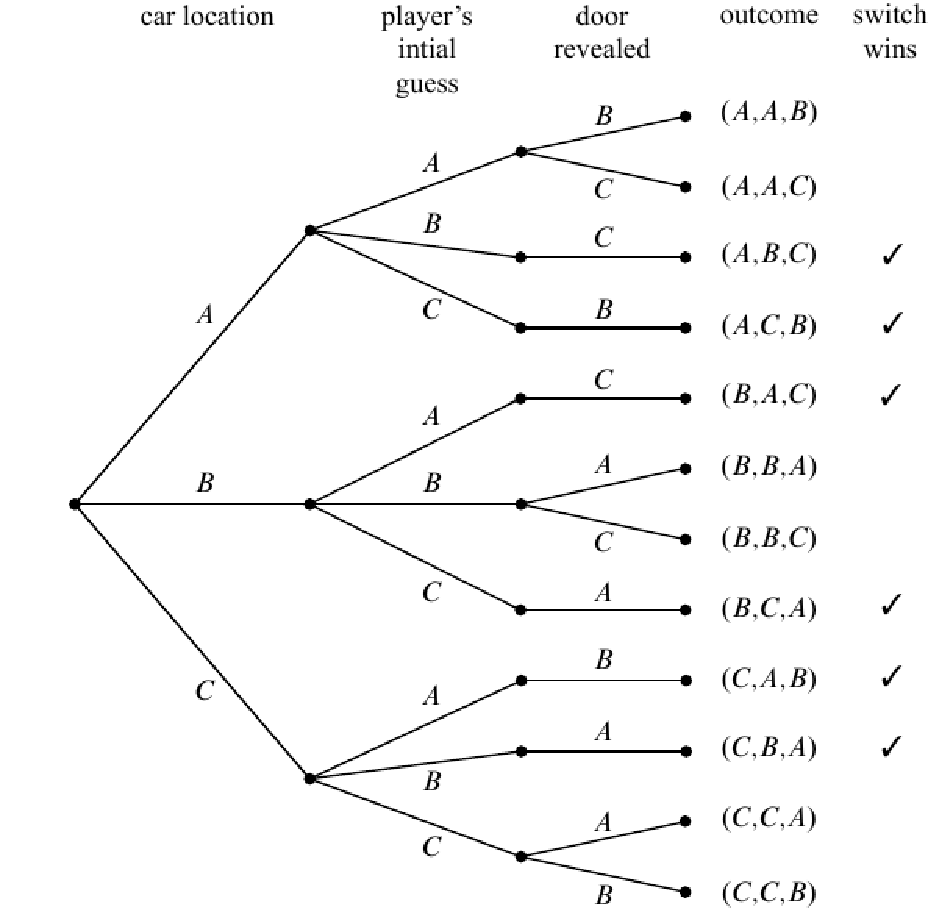
\includegraphics[scale=0.5]{fig174.pdf}
        \end{center}
      \end{block}
    %\end{center}
\end{frame}

\begin{frame}
  \begin{dfntn}
    Một \defi {không gian xác suất} bao gồm một không gian mẫu $\mathcal{S}$ và một \defi {hàm xác suất}  
    \[
   \pr[.] :\ \mathcal{S} \longrightarrow \mathbb{R}.
    \]
Hàm này  thỏa mãn:
\begin{enumerate}
\item Với mọi $w \in \mathcal{S}$,\quad  $0 \leq \pr[w] \leq 1$,
\item $\sum_{w \in \mathcal{S}}\ \pr[w] = 1 $.
\end{enumerate} 
  \end{dfntn}

$\pr[w]$ := ``Xác suất để kết quả của thử nghiệm  là  $w$''. 
\end{frame}

\begin{frame}
   % \begin{center}
      \begin{block}{}
        \begin{center}
          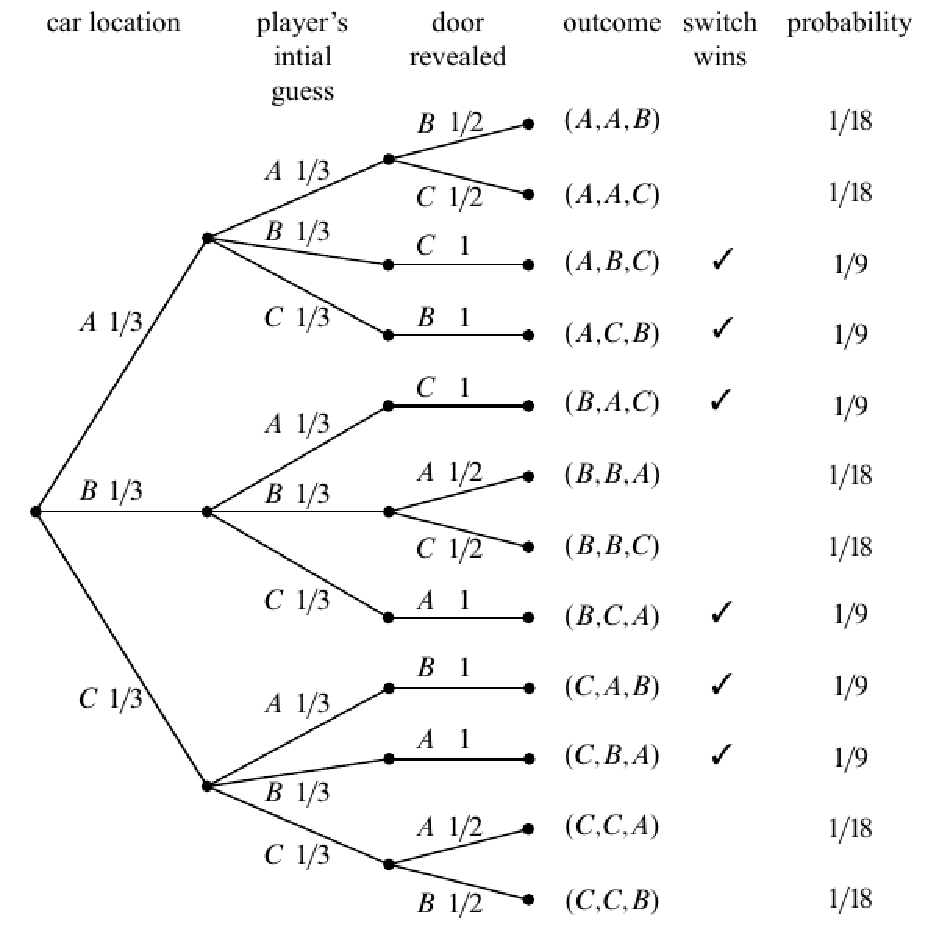
\includegraphics[scale=0.5]{fig175.pdf}
        \end{center}
      \end{block}
    %\end{center}
\end{frame}

\begin{frame}
  \begin{block}{Luật tích}
    Xác suất của một kết quả là tích của các xác suất trên đường đi trong cây dẫn đến kết quả đó.
  \end{block}
\end{frame}

\begin{frame}
  \begin{align*}
    \pr[\text{người chơi đổi  cửa mà thắng}]\ =\ ?
  \end{align*}
\end{frame}

\begin{frame}
   % \begin{center}
      \begin{block}{}
        \begin{center}
          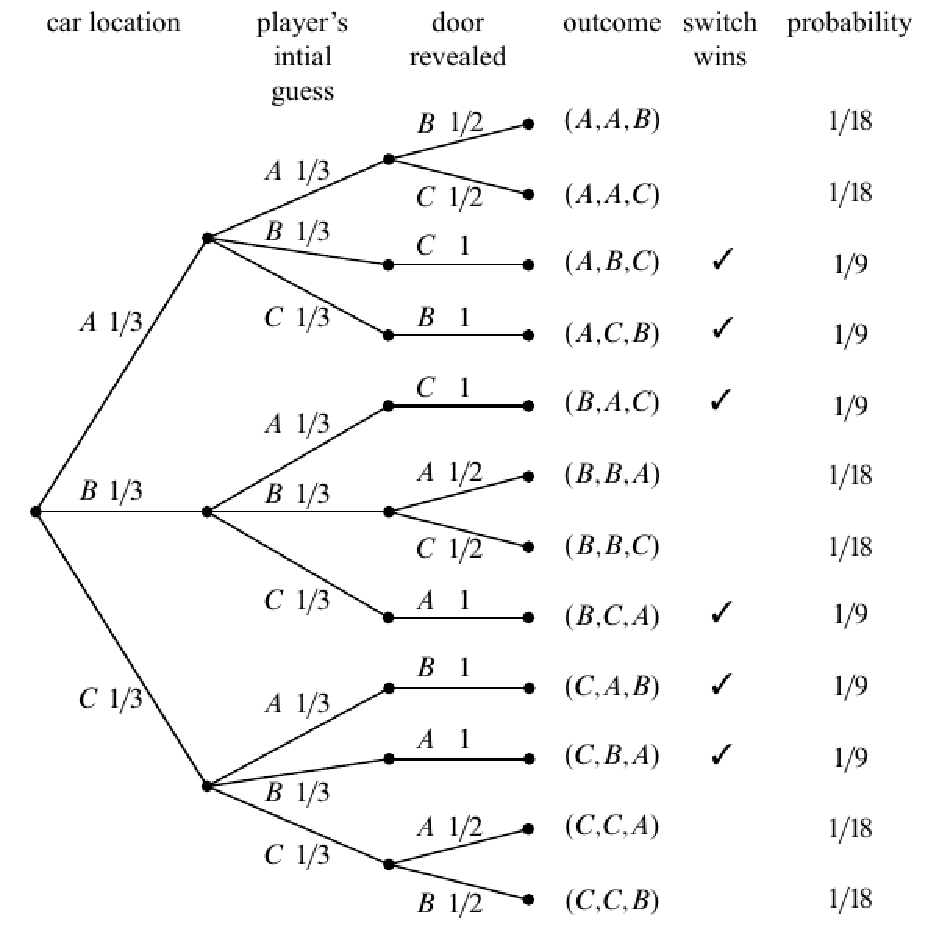
\includegraphics[scale=0.5]{fig175.pdf}
        \end{center}
      \end{block}
    %\end{center}
\end{frame}

\begin{frame}
  \begin{dfntn}
    Mỗi  \defi{sự kiện} là  một tập con của không gian mẫu.
  \end{dfntn}

  \begin{xmpl}
    $E_L = $ sự kiện người chơi thua khi chọn chiến lược ``đổi cửa''.
  \end{xmpl}
\end{frame}

\begin{frame}
  \begin{dfntn}
    Xác suất một sự kiện $E$ xuất hiện bằng 
    \[
    \pr[E] = \sum_{w \in E} \pr [w].
    \]
  \end{dfntn}

  \begin{xmpl}
    $\pr [\text{sự kiện thắng mà  không "đổi cửa"}]$ = ?
  \end{xmpl}
\end{frame}

\begin{frame}
   % \begin{center}
      \begin{block}{}
        \begin{center}
          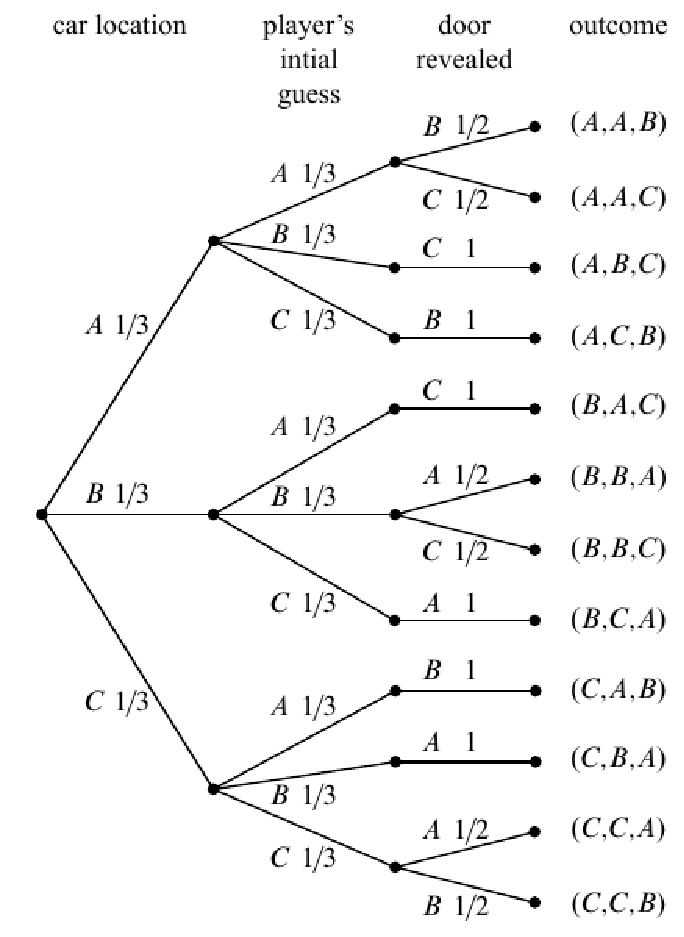
\includegraphics[scale=0.5]{fig175b.pdf}
        \end{center}
      \end{block}
    %\end{center}
\end{frame}

\section{Những con xúc xắc kỳ lạ}
\begin{frame}
  \begin{block}{Xúc xắc với các mặt đối diện bằng nhau}
    \begin{center}
      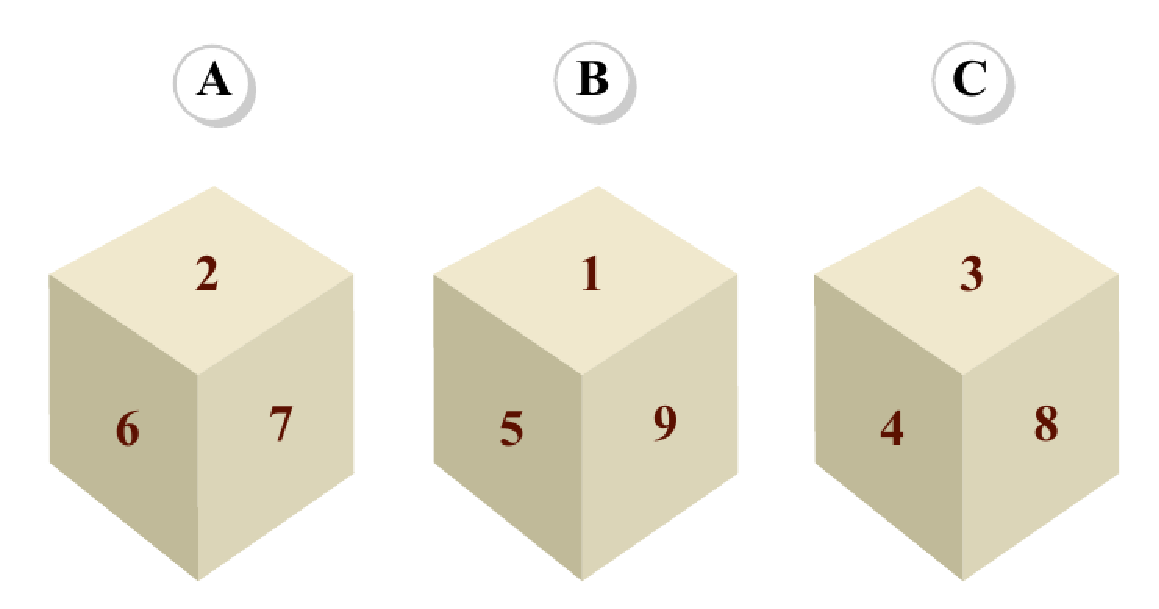
\includegraphics [scale = 0.5]{xucxac.pdf} 
    \end{center}
  \end{block}
Tôi sẽ trả bạn $105K$ nếu bạn lắc được số lớn hơn, nhưng bạn chỉ phải trả $100K$ nếu tôi được số lớn hơn. Bạn được chọn một con xúc xắc trước, tôi sẽ chọn một trong hai con còn lại. 
\end{frame}

\begin{frame}{4 bước để tính xác suất của sự kiện : $A$ thắng $B$}
  \begin{enumerate}
  \item Tìm không gian mẫu 
    $$
    \mathcal{S} = \{(2,1),(2,5),(2,9),(6,1),(6,5),(6,9), (7,1),(7,5),(7,9) \}
    $$
  \item Định nghĩa sự kiện cần quan tâm 
    $$
    \{(2,1), (6,1), (6,5), (7,1), (7,5)\}
    $$

  \item Xác định xác suất của mỗi kết quả
  \item Tính xác suất của sự kiện quan tâm
  \end{enumerate}
\end{frame}


\begin{frame}
  % \begin{center}
  \begin{block}{}
    \begin{center}
      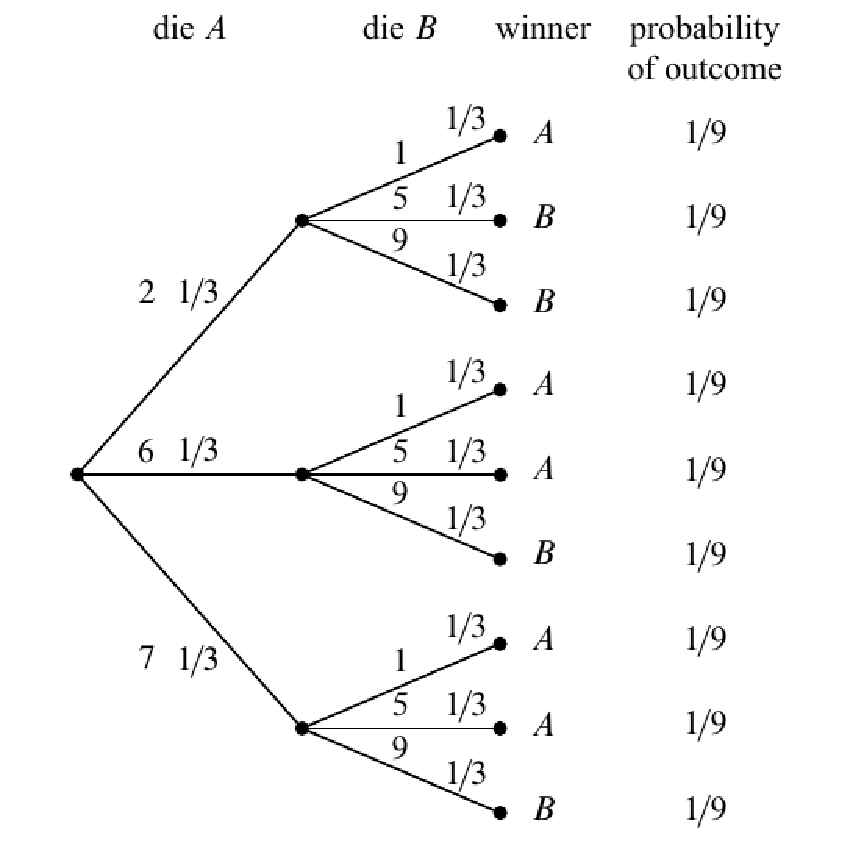
\includegraphics[scale=0.55]{fig177.pdf}
    \end{center}
  \end{block}
  % \end{center}
\end{frame}

\begin{frame}
  \begin{qstn}
    \begin{itemize}
    \item   $\pr[A \text{ thắng } B]\ =\  ?$
    \item $\pr[A \text{ thắng } C]\ =\  ?$
    \item $\pr[B \text{ thắng } C]\ =\  ?$
    \end{itemize}
  \end{qstn}
\end{frame}

\begin{frame}
  \begin{dfntn}
    Một không gian xác suất hữu hạn  $\mathcal{S}$ được gọi là \defi{đều} nếu với mọi kết quả $w \in \mathcal{S}$, ta có  $\pr[w] = 1/|\mathcal{S}|$.
  \end{dfntn}
\end{frame}

\begin{frame}
  % \begin{center}
  \begin{block}{}
    \begin{center}
      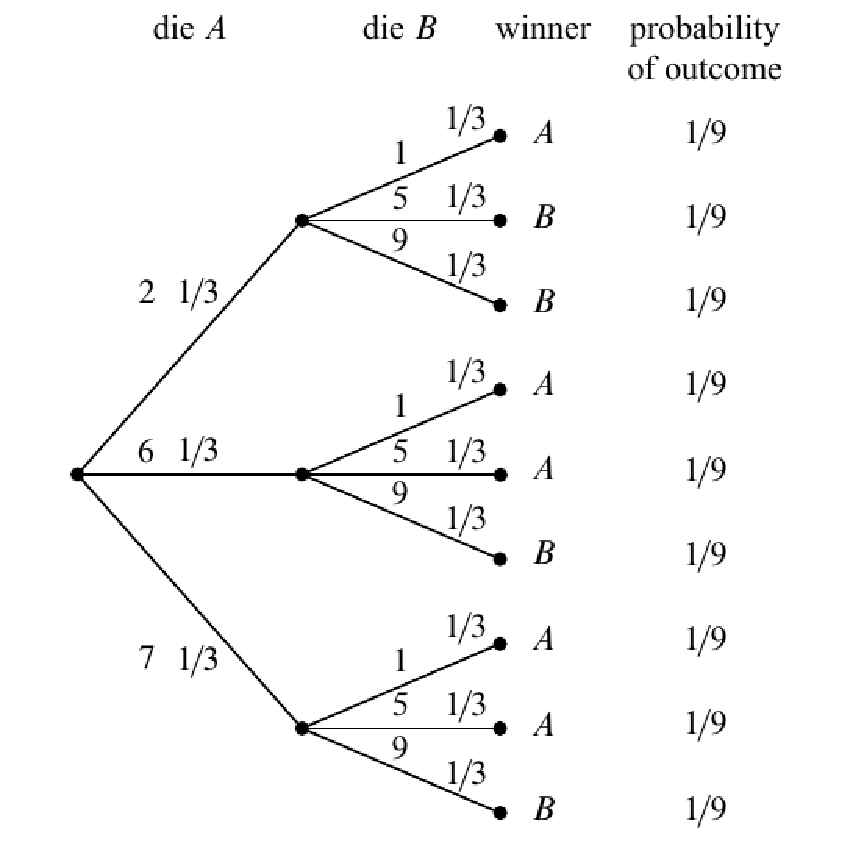
\includegraphics[scale=0.55]{fig177.pdf}
    \end{center}
  \end{block}
  % \end{center}
\end{frame}
 
\begin{frame}
  \begin{xrcs}
   Problem 3.
  \end{xrcs}
\end{frame}
\end{document}



%%% Local Variables:
%%% mode: latex
%%% TeX-master: t
%%% End:
